\documentclass[a4paper, reqno, 11pt]{amsart}
\usepackage{amsmath, amssymb, amsthm, amsfonts, mathtools}
\usepackage{graphicx, caption, xcolor, placeins}
\usepackage{color}
\usepackage{tikz}
\usetikzlibrary{arrows.meta}
\tikzset{font=\small, 
point/.style={fill, circle, inner sep=1.2pt}, % definition of points 
>={Straight Barb[round,angle=60:1.2mm 1]} % define arrows
}

\begin{document}

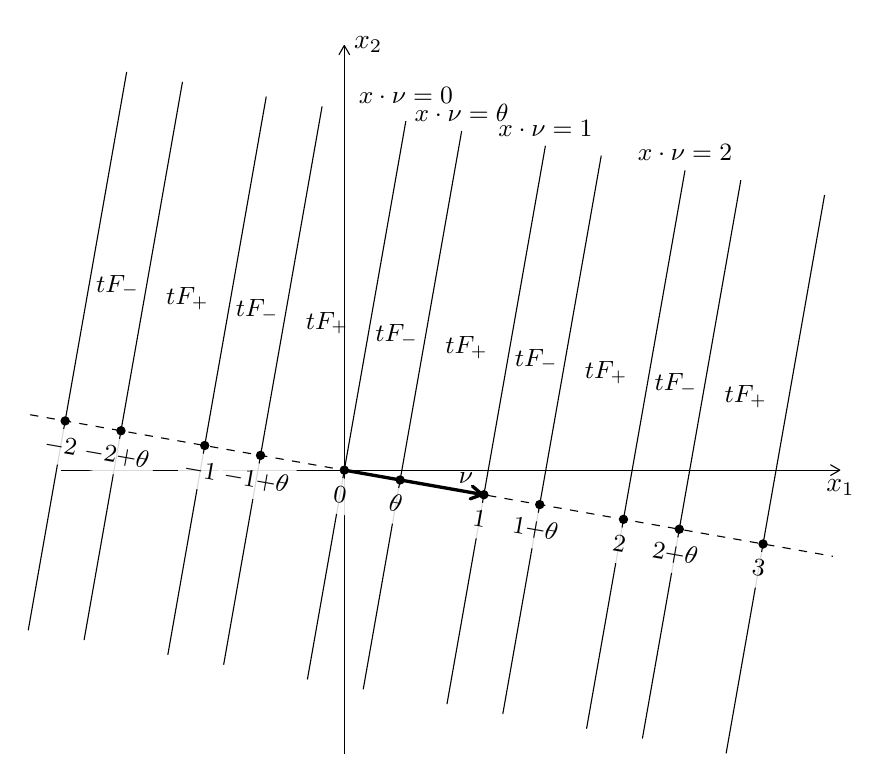
\begin{tikzpicture}[scale=1.8]%
\def\ang{-10} % degrees 
\def\th{.4}

\draw[->] (-2,0) -- (3.5,0) node[below, font=\normalsize] {$x_1$}; 
\draw[->] (0,-2) -- (0,3) node[right, font=\normalsize] {$x_2$}; 

\begin{scope}[rotate=\ang] 

\foreach \x in {-2,-1,...,2} { 
  \draw (\x,-1.5) -- (\x,0) node[point]{} -- (\x,2.5) 
    (\x+\th,-1.5) -- (\x+\th,0) node[point]{} -- (\x+\th,2.5); 
  \path (\x+\th/2,1) node{$tF_-$}  (\x+1/2+\th/2,1) node{$tF_+$}; 
  \path[every node/.style={below, fill=white, inner sep=2pt, outer sep=3pt, fill opacity=.85, text opacity=1.}] 
    (\x,0) node[rotate=\ang]{$\x\mathstrut$ } 
    (\x+\th,0) node[rotate=\ang]{\ifnum \x=0 $\theta\mathstrut$ \else $\x{+}\theta\mathstrut$ \fi}; 
}; 
\draw (3,-1.5) -- (3,0) node[point]{} 
  node[below, fill=white, inner sep=2pt, outer sep=3pt, fill opacity=.85, text opacity=1., rotate=\ang]{$3\mathstrut$} -- (3,2.5); 

\path[above] 
(0,2.5) node[yshift=1mm]{$x\cdot\nu=0$} 
(\th,2.5) node{$x\cdot\nu=\theta$} 
(1,2.5) node{$x\cdot\nu=1$} 
(2,2.5) node{$x\cdot\nu=2$}; 

\draw[->, very thick] (0,0) -- (1,0) node[above left]{$\nu$}; 
\draw[dashed] (-2.25,0) -- (3.5,0); 

\end{scope} 
\end{tikzpicture}

\end{document}